% GNUPLOT: LaTeX picture with Postscript
\begingroup
\newcommand{\ft}[0]{\footnotesize}
  \makeatletter
  \providecommand\color[2][]{%
    \GenericError{(gnuplot) \space\space\space\@spaces}{%
      Package color not loaded in conjunction with
      terminal option `colourtext'%
    }{See the gnuplot documentation for explanation.%
    }{Either use 'blacktext' in gnuplot or load the package
      color.sty in LaTeX.}%
    \renewcommand\color[2][]{}%
  }%
  \providecommand\includegraphics[2][]{%
    \GenericError{(gnuplot) \space\space\space\@spaces}{%
      Package graphicx or graphics not loaded%
    }{See the gnuplot documentation for explanation.%
    }{The gnuplot epslatex terminal needs graphicx.sty or graphics.sty.}%
    \renewcommand\includegraphics[2][]{}%
  }%
  \providecommand\rotatebox[2]{#2}%
  \@ifundefined{ifGPcolor}{%
    \newif\ifGPcolor
    \GPcolortrue
  }{}%
  \@ifundefined{ifGPblacktext}{%
    \newif\ifGPblacktext
    \GPblacktextfalse
  }{}%
  % define a \g@addto@macro without @ in the name:
  \let\gplgaddtomacro\g@addto@macro
  % define empty templates for all commands taking text:
  \gdef\gplbacktext{}%
  \gdef\gplfronttext{}%
  \makeatother
  \ifGPblacktext
    % no textcolor at all
    \def\colorrgb#1{}%
    \def\colorgray#1{}%
  \else
    % gray or color?
    \ifGPcolor
      \def\colorrgb#1{\color[rgb]{#1}}%
      \def\colorgray#1{\color[gray]{#1}}%
      \expandafter\def\csname LTw\endcsname{\color{white}}%
      \expandafter\def\csname LTb\endcsname{\color{black}}%
      \expandafter\def\csname LTa\endcsname{\color{black}}%
      \expandafter\def\csname LT0\endcsname{\color[rgb]{1,0,0}}%
      \expandafter\def\csname LT1\endcsname{\color[rgb]{0,1,0}}%
      \expandafter\def\csname LT2\endcsname{\color[rgb]{0,0,1}}%
      \expandafter\def\csname LT3\endcsname{\color[rgb]{1,0,1}}%
      \expandafter\def\csname LT4\endcsname{\color[rgb]{0,1,1}}%
      \expandafter\def\csname LT5\endcsname{\color[rgb]{1,1,0}}%
      \expandafter\def\csname LT6\endcsname{\color[rgb]{0,0,0}}%
      \expandafter\def\csname LT7\endcsname{\color[rgb]{1,0.3,0}}%
      \expandafter\def\csname LT8\endcsname{\color[rgb]{0.5,0.5,0.5}}%
    \else
      % gray
      \def\colorrgb#1{\color{black}}%
      \def\colorgray#1{\color[gray]{#1}}%
      \expandafter\def\csname LTw\endcsname{\color{white}}%
      \expandafter\def\csname LTb\endcsname{\color{black}}%
      \expandafter\def\csname LTa\endcsname{\color{black}}%
      \expandafter\def\csname LT0\endcsname{\color{black}}%
      \expandafter\def\csname LT1\endcsname{\color{black}}%
      \expandafter\def\csname LT2\endcsname{\color{black}}%
      \expandafter\def\csname LT3\endcsname{\color{black}}%
      \expandafter\def\csname LT4\endcsname{\color{black}}%
      \expandafter\def\csname LT5\endcsname{\color{black}}%
      \expandafter\def\csname LT6\endcsname{\color{black}}%
      \expandafter\def\csname LT7\endcsname{\color{black}}%
      \expandafter\def\csname LT8\endcsname{\color{black}}%
    \fi
  \fi
  \setlength{\unitlength}{0.0500bp}%
  \begin{picture}(8502.00,5102.00)%
      \csname LTb\endcsname%
      \put(4251,4882){\makebox(0,0){\strut{}Zestawienie algorytmów}}%
    \gplgaddtomacro\gplbacktext{%
      \colorrgb{0.50,0.50,0.50}%
      \put(682,751){\makebox(0,0)[r]{\strut{} 0}}%
      \colorrgb{0.50,0.50,0.50}%
      \put(682,1137){\makebox(0,0)[r]{\strut{} 5}}%
      \colorrgb{0.50,0.50,0.50}%
      \put(682,1522){\makebox(0,0)[r]{\strut{} 10}}%
      \colorrgb{0.50,0.50,0.50}%
      \put(682,1908){\makebox(0,0)[r]{\strut{} 15}}%
      \colorrgb{0.50,0.50,0.50}%
      \put(682,2293){\makebox(0,0)[r]{\strut{} 20}}%
      \colorrgb{0.50,0.50,0.50}%
      \put(682,2679){\makebox(0,0)[r]{\strut{} 25}}%
      \colorrgb{0.50,0.50,0.50}%
      \put(682,3064){\makebox(0,0)[r]{\strut{} 30}}%
      \colorrgb{0.50,0.50,0.50}%
      \put(682,3450){\makebox(0,0)[r]{\strut{} 35}}%
      \colorrgb{0.50,0.50,0.50}%
      \put(682,3835){\makebox(0,0)[r]{\strut{} 40}}%
      \colorrgb{0.50,0.50,0.50}%
      \put(682,4221){\makebox(0,0)[r]{\strut{} 45}}%
      \colorrgb{0.50,0.50,0.50}%
      \put(861,484){\makebox(0,0){\strut{}4}}%
      \colorrgb{0.50,0.50,0.50}%
      \put(1386,484){\makebox(0,0){\strut{}16}}%
      \colorrgb{0.50,0.50,0.50}%
      \put(1912,484){\makebox(0,0){\strut{}64}}%
      \colorrgb{0.50,0.50,0.50}%
      \put(2437,484){\makebox(0,0){\strut{}256}}%
      \csname LTb\endcsname%
      \put(176,1936){\rotatebox{-270}{\makebox(0,0){\strut{}Przyspieszenie}}}%
      \put(1649,154){\makebox(0,0){\strut{}Liczba procesów}}%
      \put(1649,4551){\makebox(0,0){\strut{}$n=(2048\times 2048)$}}%
    }%
    \gplgaddtomacro\gplfronttext{%
      \csname LTb\endcsname%
      \put(1701,4188){\makebox(0,0)[r]{\strut{}Cannon-DGEMM, 1 wątek}}%
      \csname LTb\endcsname%
      \put(1701,3968){\makebox(0,0)[r]{\strut{}Cannon-DGEMM, 2 wątki}}%
      \csname LTb\endcsname%
      \put(1701,3748){\makebox(0,0)[r]{\strut{}Cannon-DGEMM, 4 wątki}}%
      \csname LTb\endcsname%
      \put(1701,3528){\makebox(0,0)[r]{\strut{}Cannon-DGEMM, 12 wątków}}%
      \csname LTb\endcsname%
      \put(1701,3308){\makebox(0,0)[r]{\strut{}Cannon}}%
      \csname LTb\endcsname%
      \put(1701,3088){\makebox(0,0)[r]{\strut{}Naiwny}}%
    }%
    \gplgaddtomacro\gplbacktext{%
      \colorrgb{0.50,0.50,0.50}%
      \put(3428,751){\makebox(0,0)[r]{\strut{} 0}}%
      \colorrgb{0.50,0.50,0.50}%
      \put(3428,1137){\makebox(0,0)[r]{\strut{} 5}}%
      \colorrgb{0.50,0.50,0.50}%
      \put(3428,1522){\makebox(0,0)[r]{\strut{} 10}}%
      \colorrgb{0.50,0.50,0.50}%
      \put(3428,1908){\makebox(0,0)[r]{\strut{} 15}}%
      \colorrgb{0.50,0.50,0.50}%
      \put(3428,2293){\makebox(0,0)[r]{\strut{} 20}}%
      \colorrgb{0.50,0.50,0.50}%
      \put(3428,2679){\makebox(0,0)[r]{\strut{} 25}}%
      \colorrgb{0.50,0.50,0.50}%
      \put(3428,3064){\makebox(0,0)[r]{\strut{} 30}}%
      \colorrgb{0.50,0.50,0.50}%
      \put(3428,3450){\makebox(0,0)[r]{\strut{} 35}}%
      \colorrgb{0.50,0.50,0.50}%
      \put(3428,3835){\makebox(0,0)[r]{\strut{} 40}}%
      \colorrgb{0.50,0.50,0.50}%
      \put(3428,4221){\makebox(0,0)[r]{\strut{} 45}}%
      \colorrgb{0.50,0.50,0.50}%
      \put(3607,484){\makebox(0,0){\strut{}4}}%
      \colorrgb{0.50,0.50,0.50}%
      \put(4162,484){\makebox(0,0){\strut{}16}}%
      \colorrgb{0.50,0.50,0.50}%
      \put(4716,484){\makebox(0,0){\strut{}64}}%
      \colorrgb{0.50,0.50,0.50}%
      \put(5271,484){\makebox(0,0){\strut{}256}}%
      \csname LTb\endcsname%
      \put(4439,154){\makebox(0,0){\strut{}Liczba procesów}}%
      \put(4439,4551){\makebox(0,0){\strut{}$n=(4096\times 4096)$}}%
    }%
    \gplgaddtomacro\gplfronttext{%
    }%
    \gplgaddtomacro\gplbacktext{%
      \colorrgb{0.50,0.50,0.50}%
      \put(6262,751){\makebox(0,0)[r]{\strut{} 0}}%
      \colorrgb{0.50,0.50,0.50}%
      \put(6262,1137){\makebox(0,0)[r]{\strut{} 5}}%
      \colorrgb{0.50,0.50,0.50}%
      \put(6262,1522){\makebox(0,0)[r]{\strut{} 10}}%
      \colorrgb{0.50,0.50,0.50}%
      \put(6262,1908){\makebox(0,0)[r]{\strut{} 15}}%
      \colorrgb{0.50,0.50,0.50}%
      \put(6262,2293){\makebox(0,0)[r]{\strut{} 20}}%
      \colorrgb{0.50,0.50,0.50}%
      \put(6262,2679){\makebox(0,0)[r]{\strut{} 25}}%
      \colorrgb{0.50,0.50,0.50}%
      \put(6262,3064){\makebox(0,0)[r]{\strut{} 30}}%
      \colorrgb{0.50,0.50,0.50}%
      \put(6262,3450){\makebox(0,0)[r]{\strut{} 35}}%
      \colorrgb{0.50,0.50,0.50}%
      \put(6262,3835){\makebox(0,0)[r]{\strut{} 40}}%
      \colorrgb{0.50,0.50,0.50}%
      \put(6262,4221){\makebox(0,0)[r]{\strut{} 45}}%
      \colorrgb{0.50,0.50,0.50}%
      \put(6441,484){\makebox(0,0){\strut{}4}}%
      \colorrgb{0.50,0.50,0.50}%
      \put(6996,484){\makebox(0,0){\strut{}16}}%
      \colorrgb{0.50,0.50,0.50}%
      \put(7550,484){\makebox(0,0){\strut{}64}}%
      \colorrgb{0.50,0.50,0.50}%
      \put(8105,484){\makebox(0,0){\strut{}256}}%
      \csname LTb\endcsname%
      \put(7273,154){\makebox(0,0){\strut{}Liczba procesów}}%
      \put(7273,4551){\makebox(0,0){\strut{}$n=(8192\times 8192)$}}%
    }%
    \gplgaddtomacro\gplfronttext{%
    }%
    \gplbacktext
    \put(0,0){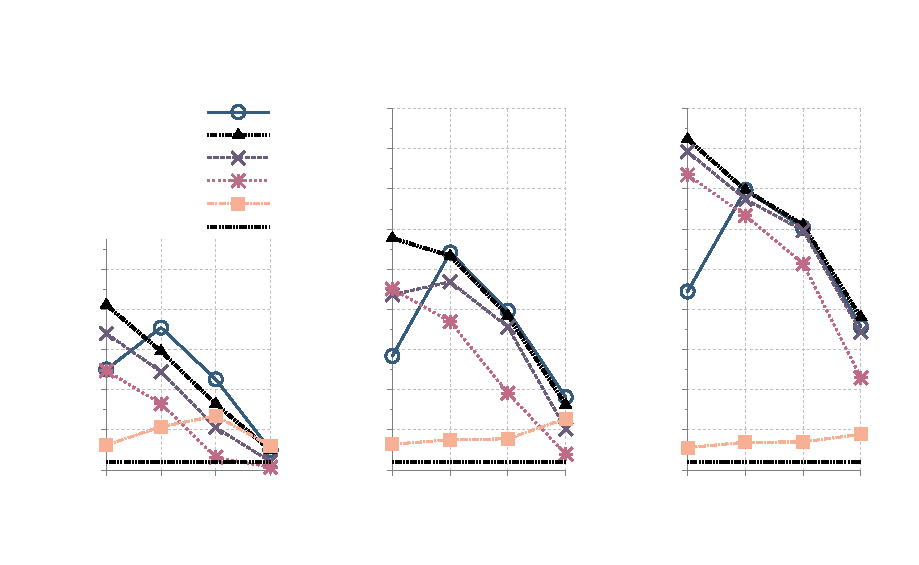
\includegraphics{cannon_dgemm}}%
    \gplfronttext
  \end{picture}%
\endgroup
